\documentclass[prl,twocolumn]{revtex4-1}

\usepackage{graphicx}
\usepackage{color}
\usepackage{latexsym,amsmath}

\definecolor{linkcolor}{rgb}{0,0,0.65} %hyperlink
\usepackage[pdftex,colorlinks=true, pdfstartview=FitV, linkcolor= linkcolor, citecolor= linkcolor, urlcolor= linkcolor, hyperindex=true,hyperfigures=true]{hyperref} %hyperlink%

\makeatletter
\renewcommand{\section}{\@startsection{section}{1}{\z@}%
	{-3.5ex \@plus -1ex \@minus -.2ex}{2.3ex \@plus.2ex}%
	{\normalfont\bfseries\raggedright}}
\makeatother



\begin{document}

\title{GROUP2505 -- Log-likelihood analysis for Restricted Boltzmann Machines}





\author{Elias Maria Bonasera}
\author{Alberto Casellato}
\author{Nicola Garbin}
\author{Francesco Pazzocco (781238?)}

\date{\today}


\begin{abstract}
  Here, in the ``abstract'' (more or less of 8 lines), there should be a short summary of the work and of its main findings. In a paper, the abstract is important also for attracting potential readers, hence it is convenient to start it with some catchy statement. ---
 The rest of this text has the double purpose of (a) providing a template for the assignment latex, and (b) introducing how to structure the backbone of the text and explaining some details of this assignment. The ``zzz'' fill the space to show a typical (but not rigid) extension of the parts.
  zzzzzzzzzzzzzzz zzzzz zzzzzzzzzz zzzzzzz z zzzzzzzzzzz zzzz zzzzzzzzz
  zzzzzzzzzzzzzzz zzzzz zzzzzzzzzz zzzzzzz z zzzzzzzzzzz zzzz zzzzzzzzz
  zzzzzzzzzzzzzzz zzzzz zzzzzzzzzz zzzzzzz z zzzzzzzzzzz zzzz zzzzzzzzz
  zzzzzzzzzzzzzzz zzzzz zzzzzzzzzz zzzzzzz z zzzzzzzzzzz zzzz zzzzzzzzz.
\end{abstract}

\maketitle


\section{1. Introduction}

The main goal of this assignment is to explore how the performance of an RBM changes for different choices of the hyperparameters of the model, using the MNIST digits as the database; in particular using the log-likelihood evaluation we explore the trend of the model during the learning process as the number of epochs increases.

Restricted Boltzmann Machines (RBM) are a powerful kind of generative models designed to accomplish training processes relatively fast. In RBMs, a set of binary visible units $i$ of state $v_i$ is symmetrically connected to a set of binary hidden units $\mu$ of state $h_\mu$; the continuos weight $w_{i\mu}$ quantifies the strength between unit $i$ and unit $\mu$ (see Figure~\ref{fig:RBM_architecture}). RBMs use an energy function to define the probability distribution over the input data. In the training process the energy of the configuration is minimized by adjusting the parameters $\theta$. The most common training algorithm is contrastive divergence which allows to approximate the gradient of the likelihood to update the parameters. During this process, a cyclic Gibbs sampling is performed setting the visible units given the hidden ones and vice versa, according to the following probabilities:

\begin{equation}
	p(h_\mu=1\ |\ \mathbf{v}) = \sigma(b_\mu + \sum_{i}v_iw_{i\mu})
	\label{eq:p_of_h}
\end{equation}
\begin{equation}
	p(v_i=1\ |\ \mathbf{h}) = \sigma(a_i + \sum_{\mu}h_{\mu}w_{i\mu})
	\label{eq:p_of_v}
\end{equation}

where $\sigma(x)=1/(1+e^{-x})$ is the logistic sigmoid function, $a_i$ is the bias of the $i$-th visible unit and $b_\mu$ is the bias of the $\mu$-th hidden unit; they act shifting the sigmoid function $\sigma(x)$. The absence of links among units of the same type simplifies the training process. Moreover, the number of iterations of Eq.~\ref{eq:p_of_h} and Eq.~\ref{eq:p_of_v} can be setted to $1$ if real data is used to fix $\mathbf{v}$ in the first place.
\\
\\
\\
The goodness of the models is evaluated by computing the log-likelihood $\mathcal{L}$ of the data:

\begin{equation}
	\mathcal{L}=\frac{1}{M}\sum_{m=1}^{M}{\mathfrak{l}_{\theta}(v^{(m)})}
	\label{eq:Loglikelihood}
\end{equation}
\begin{equation}
	\mathfrak{l}_{\theta}(v^{(m)})=\log\sum_{h}{e^{-E(v,h)}-\log{Z}}
	\label{eq:loglikelihood}
\end{equation}

where $M$ is the number of data points, $E(v,h)$ is the energy function, $Z$ is the partition function and, in Eq.~\ref{eq:loglikelihood}, the index $h$ of the summation represents each possible state of the hidden layer.

%%%%%%%%%%%%%%%%%%%
\begin{figure}[!tb]
	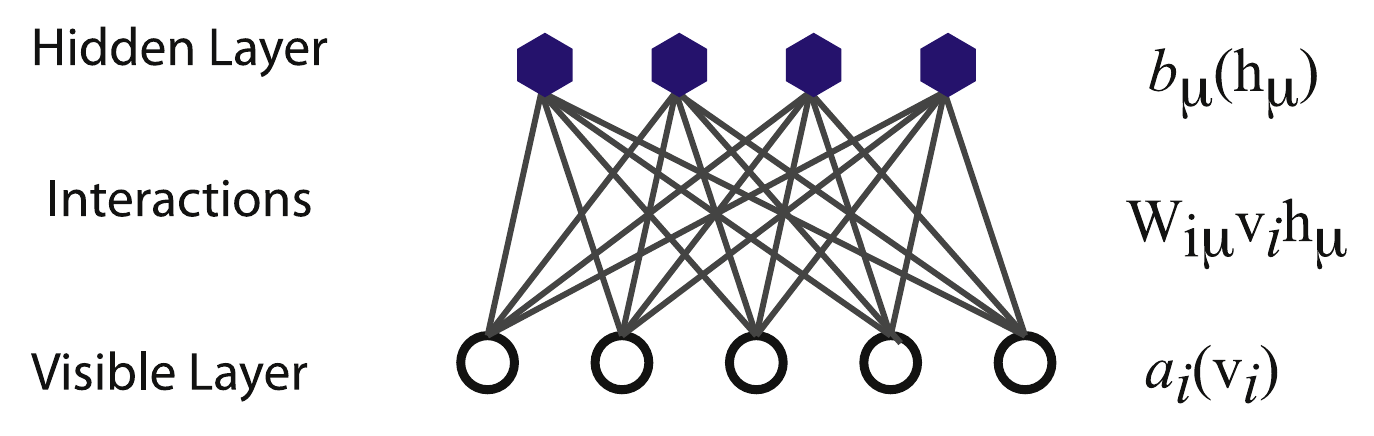
\includegraphics[width=0.44\textwidth]{RBM_structure.png}
	\caption{A Restricted Boltzmann Machine (RBM) is made up of visible units, denoted as $v_i$, and hidden units, represented as $h_\mu$. These units engage with one another through interactions characterized by the weights $W_{i\mu}$. Notably, there are no direct interactions among the visible units or among the hidden units themselves.}
	\label{fig:RBM_architecture}
\end{figure}
%%%%%%%%%%%%%%%%%%%


The topic of your assignment is specified at the lesson.
It requires you to describe your findings in one of the exercises.

In this introduction,
you should describe the main topic in general terms, introducing what you want to discover, why, and which
methods you use do perform this study.
There could also be citations like this \cite{pap1} to papers, websites, etc. forming the list of references that other people could be interested in consulting for a better understanding your points.

\paragraph{\bf Tips}
\begin{itemize}
\item In English use sentences shorter than what you might normally be using in Italian, German, etc...
\item Possibly, Explain concepts at a level which is accessible to everybody.
\item Do not use colloquial forms in scientific writing, thus avoid it's, aren't, don't, etc.
\item Do not change the time of verbs; it is simpler to speak in simple present, however also writing always in past tense is fine.
\item In figures, use fonts that match the \underline{size} of the main text fonts (tiny fonts should be avoided). Use lines with different dashing, color, and symbol as appropriate for better distinguishing the curves. Use log scale when it is better for highlighting smaller scales or flattening larger scales. 
\item Remember the grid explained in the intro video of the course, which will be used for evaluations. It contains suggestions for improving the text.
\end{itemize}




\paragraph{\bf Latex --}

A modern online tool to handle and share latex files is {\em Overleaf}. The other option is a standard latex installation on the computer.
Locally, this text is compiled with the command \texttt{pdflatex} and is based on \texttt{revtex}.
Packages (of which, maybe not all are needed) in Arch Linux may be installed via\\
\texttt{
  sudo pacman -S texlive-core texlive-bibtexextra texlive-fontsextra  texlive-formatsextra texlive-latexextra texlive-pictures texlive-pstricks texlive-publishers  texlive-science}

\vspace{0.2cm}
In Ubuntu there is a similar installation with \texttt{sudo apt install}, maybe \texttt{sudo apt install texlive-full} if you want to lose less time to pick the right packages. Similar tools should be available in Windows and via e.g.~macports on Mac OS.

%%%%%%%%%%%%%%%%%%%
\begin{figure*}[!tb]
  \centering
  
\includegraphics[width=0.3\textwidth]{fig1a.png}
  \hskip 1mm
  
\includegraphics[width=0.3\textwidth]{fig1a.png}
  \hskip 1mm
  
\includegraphics[width=0.3\textwidth]{fig1a.png}
  \vskip 1mm
  
\includegraphics[width=0.455\textwidth]{fig1a.png}
  \hskip 1mm
  
\includegraphics[width=0.455\textwidth]{fig1a.png}
  \caption{Description of the panels: (a)..... (b)... etc. This caption should give enough info on the content of figures to make them mostly readable without consulting the main text. However, repetitions with the main text should e avoided if possible. {\color{red} If this format is difficult to frame in the page you want, just break it into multiple single figures.}}
  \label{fig:x}
\end{figure*}
%%%%%%%%%%%%%%%%%%%

\section{2. Methods}
\subsection{2.1. Theory}

Concerning the training process of RBM, $\mathbf{v}$ is setted using real data. Weights $w_{i\mu}$ are initialized sampling values from a Gaussian distribution of mean $0$ and standard deviation $0.01$. Biases $b_\mu$ of hidden units are initialized to $0$. Thus $\mathbf{h}$ is evaluated by Eq.~\ref{eq:p_of_h} before passed to Eq.~\ref{eq:p_of_v} in order to compute back $\mathbf{v}$. In such evaluation it is convenient to set $a_i=\log[p_i/(1-p_i)]$; fixed the $i$-th visible unit, $p_i$ is defined as the number of times such unit is on over the whole training array set, normalized over the size of the set. Referring to Eq.~\ref{eq:p_of_v}, the choice of shifting the sigmoid $\sigma(x)$ by the function $\log[p_i/(1-p_i)]$ of the average $p_i$ ensures that the units can activate properly, even given initial weights $w_{i\mu}$ close to $0$.

The initialization of biases $a_i$, firstly proposed by Hinton, makes hidden units able to activate and differentiate better their activation based on data, avoiding the risk of getting stuck on values near to $0$.

\subsection{2.2. Computation}





 Here describe which tools you decided to use for solving the problem, with
 equations
\begin{equation}
  A=B
  \label{eq:simple}
\end{equation}
or systems of equations
\begin{align}
  \dot v(t) & =  -U'(x)\nonumber \\
  \dot x(t) & =  v(t)
  \label{eq:motion}
\end{align}
and  eventually with  pieces of code
%%%%%%%%%%%%%%%%%%%
\begin{figure}[h]
  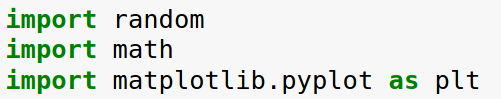
\includegraphics[width=0.7\columnwidth]{line1.png}
\end{figure}
%%%%%%%%%%%%%%%%%%%
(Jupyter allows saving in latex, it might produce a better output than including a figure with the code as done here).

  As already mentioned, the rest of the text is filled with ``zzz'' to show the typical length of the corresponding sections.


  zzzzzzzzzzzzzzz zzzzz zzzzzzzzzz zzzzzzz z zzzzzzzzzzz zzzz zzzzzzzzz
  zzzzzzzzzzzzzzz zzzzz zzzzzzzzzz zzzzzzz z zzzzzzzzzzz zzzz zzzzzzzzz.
  zzzzzzzzzzzzzzz zzzzz zzzzzzzzzz zzzzzzz z zzzzzzzzzzz zzzz zzzzzzzzz
  zzzzzzzzzzzzzzz zzzzz zzzzzzzzzz zzzzzzz z zzzzzzzzzzz zzzz zzzzzzzzz
  zzzzzzzzzzzzzzz zzzzz zzzzzzzzzz zzzzzzz z zzzzzzzzzzz zzzz zzzzzzzzz
  zzzzzzzzzzzzzzz zzzzz zzzzzzzzzz zzzzzzz z zzzzzzzzzzz zzzz zzzzzzzzz
  zzzzzzzzzzzzzzz zzzzz zzzzzzzzzz zzzzzzz z zzzzzzzzzzz zzzz zzzzzzzzz.


  
%%%%%%%%%%%%%%%%%%%%%%%%%%%%%%%%%%%%%%%%%%%%%%%%%%%%%%%%%%%%%%%%%%% 
\begin{table}[!b]
\begin{center}
\begin{tabular}{lll}
quantity & symbol & dimensionless \\
\hline
time & $t$ & $t'$  \\
momentum & $p$ & $v$
\end{tabular}
\end{center}
\caption{Description of the table.}
\label{tab:1}
\end{table}
%%%%%%%%%%%%%%%%%%%%%%%%%%%%%%%%%%%%%%%%%%%%%%%%%%%%%%%%%%%%%%%%%%%


  
  zzzzzzzzzzzzzzz zzzzz zzzzzzzzzz zzzzzzz z zzzzzzzzzzz zzzz zzzzzzzzz
  zzzzzzzzzzzzzzz zzzzz zzzzzzzzzz zzzzzzz z zzzzzzzzzzz zzzz zzzzzzzzz
  zzzzzzzzzzzzzzz zzzzz zzzzzzzzzz zzzzzzz z zzzzzzzzzzz zzzz zzzzzzzzz
  zzzzzzzzzzzzzzz zzzzz zzzzzzzzzz zzzzzzz z zzzzzzzzzzz zzzz zzzzzzzzz
  zzzzzzzzzzzzzzz zzzzz zzzzzzzzzz zzzzzzz z zzzzzzzzzzz zzzz zzzzzzzzz.


  zzzzzzzzzzzzzzz zzzzz zzzzzzzzzz zzzzzzz z zzzzzzzzzzz zzzz zzzzzzzzz
  zzzzzzzzzzzzzzz zzzzz zzzzzzzzzz zzzzzzz z zzzzzzzzzzz zzzz zzzzzzzzz
  zzzzzzzzzzzzzzz zzzzz zzzzzzzzzz zzzzzzz z zzzzzzzzzzz zzzz zzzzzzzzz
  zzzzzzzzzzzzzzz zzzzz zzzzzzzzzz zzzzzzz z zzzzzzzzzzz zzzz zzzzzzzzz
  zzzzzzzzzzzzzzz zzzzz zzzzzzzzzz zzzzzzz z zzzzzzzzzzz zzzz zzzzzzzzz.
  zzzzzzzzzzzzzzz zzzzz zzzzzzzzzz zzzzzzz z zzzzzzzzzzz zzzz zzzzzzzzz
  zzzzzzzzzzzzzzz zzzzz zzzzzzzzzz zzzzzzz z zzzzzzzzzzz zzzz zzzzzzzzz
  zzzzzzzzzzzzzzz zzzzz zzzzzzzzzz zzzzzzz z zzzzzzzzzzz zzzz zzzzzzzzz.
 


\section{3. Results}


Describe what you found.

Cite Figure~\ref{fig:x}(a), etc. to add information. Later also cite Figure~\ref{fig:y} and  Figure~\ref{fig:z}. Of course the number and size of figures may vary from project to project.

Cite Table~\ref{tab:1} to collect useful data in a clear way.

  zzzzzzzzzzzzzzz zzzzz zzzzzzzzzz zzzzzzz z zzzzzzzzzzz zzzz zzzzzzzzz
  zzzzzzzzzzzzzzz zzzzz zzzzzzzzzz zzzzzzz z zzzzzzzzzzz zzzz zzzzzzzzz
  zzzzzzzzzzzzzzz zzzzz zzzzzzzzzz zzzzzzz z zzzzzzzzzzz zzzz zzzzzzzzz
  zzzzzzzzzzzzzzz zzzzz zzzzzzzzzz zzzzzzz z zzzzzzzzzzz zzzz zzzzzzzzz
  zzzzzzzzzzzzzzz zzzzz zzzzzzzzzz zzzzzzz z zzzzzzzzzzz zzzz zzzzzzzzz.

  zzzzzzzzzzzzzzz zzzzz zzzzzzzzzz zzzzzzz z zzzzzzzzzzz zzzz zzzzzzzzz
  zzzzzzzzzzzzzzz zzzzz zzzzzzzzzz zzzzzzz z zzzzzzzzzzz zzzz zzzzzzzzz
  zzzzzzzzzzzzzzz zzzzz zzzzzzzzzz zzzzzzz z zzzzzzzzzzz zzzz zzzzzzzzz
  zzzzzzzzzzzzzzz zzzzz zzzzzzzzzz zzzzzzz z zzzzzzzzzzz zzzz zzzzzzzzz
  zzzzzzzzzzzzzzz zzzzz zzzzzzzzzz zzzzzzz z zzzzzzzzzzz zzzz zzzzzzzzz.
  zzzzzzzzzzzzzzz zzzzz zzzzzzzzzz zzzzzzz z zzzzzzzzzzz zzzz zzzzzzzzz
  zzzzzzzzzzzzzzz zzzzz zzzzzzzzzz zzzzzzz z zzzzzzzzzzz zzzz zzzzzzzzz
  zzzzzzzzzzzzzzz zzzzz zzzzzzzzzz zzzzzzz z zzzzzzzzzzz zzzz zzzzzzzzz
  zzzzzzzzzzzzzzz zzzzz zzzzzzzzzz zzzzzzz z zzzzzzzzzzz zzzz zzzzzzzzz
  zzzzzzzzzzzzzzz zzzzz zzzzzzzzzz zzzzzzz z zzzzzzzzzzz zzzz zzzzzzzzz.
  
%%%%%%%%%%%%%%%%%%%
\begin{figure}[!tb]
  
\includegraphics[width=0.44\textwidth]{fig1a.png}
  \caption{Description...}
  \label{fig:y}
\end{figure}
%%%%%%%%%%%%%%%%%%%

  zzzzzzzzzzzzzzz zzzzz zzzzzzzzzz zzzzzzz z zzzzzzzzzzz zzzz zzzzzzzzz
  zzzzzzzzzzzzzzz zzzzz zzzzzzzzzz zzzzzzz z zzzzzzzzzzz zzzz zzzzzzzzz
  zzzzzzzzzzzzzzz zzzzz zzzzzzzzzz zzzzzzz z zzzzzzzzzzz zzzz zzzzzzzzz
  zzzzzzzzzzzzzzz zzzzz zzzzzzzzzz zzzzzzz z zzzzzzzzzzz zzzz zzzzzzzzz
  zzzzzzzzzzzzzzz zzzzz zzzzzzzzzz zzzzzzz z zzzzzzzzzzz zzzz zzzzzzzzz.

  

  zzzzzzzzzzzzzzz zzzzz zzzzzzzzzz zzzzzzz z zzzzzzzzzzz zzzz zzzzzzzzz
  zzzzzzzzzzzzzzz zzzzz zzzzzzzzzz zzzzzzz z zzzzzzzzzzz zzzz zzzzzzzzz
  zzzzzzzzzzzzzzz zzzzz zzzzzzzzzz zzzzzzz z zzzzzzzzzzz zzzz zzzzzzzzz
  zzzzzzzzzzzzzzz zzzzz zzzzzzzzzz zzzzzzz z zzzzzzzzzzz zzzz zzzzzzzzz
  zzzzzzzzzzzzzzz zzzzz zzzzzzzzzz zzzzzzz z zzzzzzzzzzz zzzz zzzzzzzzz.
  
%%%%%%%%%%%%%%%%%%%
\begin{figure}[!tb]
  
\includegraphics[width=0.44\textwidth]{fig1a.png}
  \caption{Description...}
  \label{fig:z}
\end{figure}
%%%%%%%%%%%%%%%%%%%


  zzzzzzzzzzzzzzz zzzzz zzzzzzzzzz zzzzzzz z zzzzzzzzzzz zzzz zzzzzzzzz
  zzzzzzzzzzzzzzz zzzzz zzzzzzzzzz zzzzzzz z zzzzzzzzzzz zzzz zzzzzzzzz
  zzzzzzzzzzzzzzz zzzzz zzzzzzzzzz zzzzzzz z zzzzzzzzzzz zzzz zzzzzzzzz
  zzzzzzzzzzzzzzz zzzzz zzzzzzzzzz zzzzzzz z zzzzzzzzzzz zzzz zzzzzzzzz
  zzzzzzzzzzzzzzz zzzzz zzzzzzzzzz zzzzzzz z zzzzzzzzzzz zzzz zzzzzzzzz.
  zzzzzzzzzzzzzzz zzzzz zzzzzzzzzz zzzzzzz z zzzzzzzzzzz zzzz zzzzzzzzz
  zzzzzzzzzzzzzzz zzzzz zzzzzzzzzz zzzzzzz z zzzzzzzzzzz zzzz zzzzzzzzz
  zzzzzzzzzzzzzzz zzzzz zzzzzzzzzz zzzzzzz z zzzzzzzzzzz zzzz zzzzzzzzz
  zzzzzzzzzzzzzzz zzzzz zzzzzzzzzz zzzzzzz z zzzzzzzzzzz zzzz zzzzzzzzz
  zzzzzzzzzzzzzzz zzzzz zzzzzzzzzz zzzzzzz z zzzzzzzzzzz zzzz zzzzzzzzz.
  
  zzzzzzzzzzzzzzz zzzzz zzzzzzzzzz zzzzzzz z zzzzzzzzzzz zzzz zzzzzzzzz
  zzzzzzzzzzzzzzz zzzzz zzzzzzzzzz zzzzzzz z zzzzzzzzzzz zzzz zzzzzzzzz
  zzzzzzzzzzzzzzz zzzzz zzzzzzzzzz zzzzzzz z zzzzzzzzzzz zzzz zzzzzzzzz
  zzzzzzzzzzzzzzz zzzzz zzzzzzzzzz zzzzzzz z zzzzzzzzzzz zzzz zzzzzzzzz
  zzzzzzzzzzzzzzz zzzzz zzzzzzzzzz zzzzzzz z zzzzzzzzzzz zzzz zzzzzzzzz.

  


  zzzzzzzzzzzzzzz zzzzz zzzzzzzzzz zzzzzzz z zzzzzzzzzzz zzzz zzzzzzzzz
  zzzzzzzzzzzzzzz zzzzz zzzzzzzzzz zzzzzzz z zzzzzzzzzzz zzzz zzzzzzzzz
  zzzzzzzzzzzzzzz zzzzz zzzzzzzzzz zzzzzzz z zzzzzzzzzzz zzzz zzzzzzzzz
  zzzzzzzzzzzzzzz zzzzz zzzzzzzzzz zzzzzzz z zzzzzzzzzzz zzzz zzzzzzzzz
  zzzzzzzzzzzzzzz zzzzz zzzzzzzzzz zzzzzzz z zzzzzzzzzzz zzzz zzzzzzzzz.

\section{4. Conclusions}

Discuss the key aspects that we can take home from this work.

Check if your text is light, swift, and correct in exposing its passages.

  zzzzzzzzzzzzzzz zzzzz zzzzzzzzzz zzzzzzz z zzzzzzzzzzz zzzz zzzzzzzzz
  zzzzzzzzzzzzzzz zzzzz zzzzzzzzzz zzzzzzz z zzzzzzzzzzz zzzz zzzzzzzzz
  zzzzzzzzzzzzzzz zzzzz zzzzzzzzzz zzzzzzz z zzzzzzzzzzz zzzz zzzzzzzzz
  zzzzzzzzzzzzzzz zzzzz zzzzzzzzzz zzzzzzz z zzzzzzzzzzz zzzz zzzzzzzzz.
  zzzzzzzzzzzzzzz zzzzz zzzzzzzzzz zzzzzzz z zzzzzzzzzzz zzzz zzzzzzzzz
  zzzzzzzzzzzzzzz zzzzz zzzzzzzzzz zzzzzzz z zzzzzzzzzzz zzzz zzzzzzzzz.

  
  zzzzzzzzzzzzzzz zzzzz zzzzzzzzzz zzzzzzz z zzzzzzzzzzz zzzz zzzzzzzzz
  zzzzzzzzzzzzzzz zzzzz zzzzzzzzzz zzzzzzz z zzzzzzzzzzz zzzz zzzzzzzzz
  zzzzzzzzzzzzzzz zzzzz zzzzzzzzzz zzzzzzz z zzzzzzzzzzz zzzz zzzzzzzzz
  zzzzzzzzzzzzzzz zzzzz zzzzzzzzzz zzzzzzz z zzzzzzzzzzz zzzz zzzzzzzzz
  zzzzzzzzzzzzzzz zzzzz zzzzzzzzzz zzzzzzz z zzzzzzzzzzz zzzz zzzzzzzzz.
  
  zzzzzzzzzzzzzzz zzzzz zzzzzzzzzz zzzzzzz z zzzzzzzzzzz zzzz zzzzzzzzz
  zzzzzzzzzzzzzzz zzzzz zzzzzzzzzz zzzzzzz z zzzzzzzzzzz zzzz zzzzzzzzz.

  
  
  zzzzzzzzzzzzzzz zzzzz zzzzzzzzzz zzzzzzz z zzzzzzzzzzz zzzz zzzzzzzzz
  zzzzzzzzzzzzzzz zzzzz zzzzzzzzzz zzzzzzz z zzzzzzzzzzz zzzz zzzzzzzzz
  zzzzzzzzzzzzzzz zzzzz zzzzzzzzzz zzzzzzz z zzzzzzzzzzz zzzz zzzzzzzzz
  zzzzzzzzzzzzzzz zzzzz zzzzzzzzzz zzzzzzz z zzzzzzzzzzz zzzz zzzzzzzzz
  zzzzzzzzzzzzzzz zzzzz zzzzzzzzzz zzzzzzz z zzzzzzzzzzz zzzz zzzzzzzzz.
  
  zzzzzzzzzzzzzzz zzzzz zzzzzzzzzz zzzzzzz z zzzzzzzzzzz zzzz zzzzzzzzz
  zzzzzzzzzzzzzzz zzzzz zzzzzzzzzz zzzzzzz z zzzzzzzzzzz zzzz zzzzzzzzz.

  





\begin{thebibliography}{99}

\bibitem{pap1}
  B. Franklin,
  J. Here There {\bf 10}, 20--40 (1800).
  
\bibitem{pap2}
  A. Einstein,
  Int. J. There Here {\bf 20}, 125--133 (1910).
  
\end{thebibliography}

\clearpage

%%%%%%%%%%%%%%%%%%%
\begin{figure*}[!tb]
  \centering
  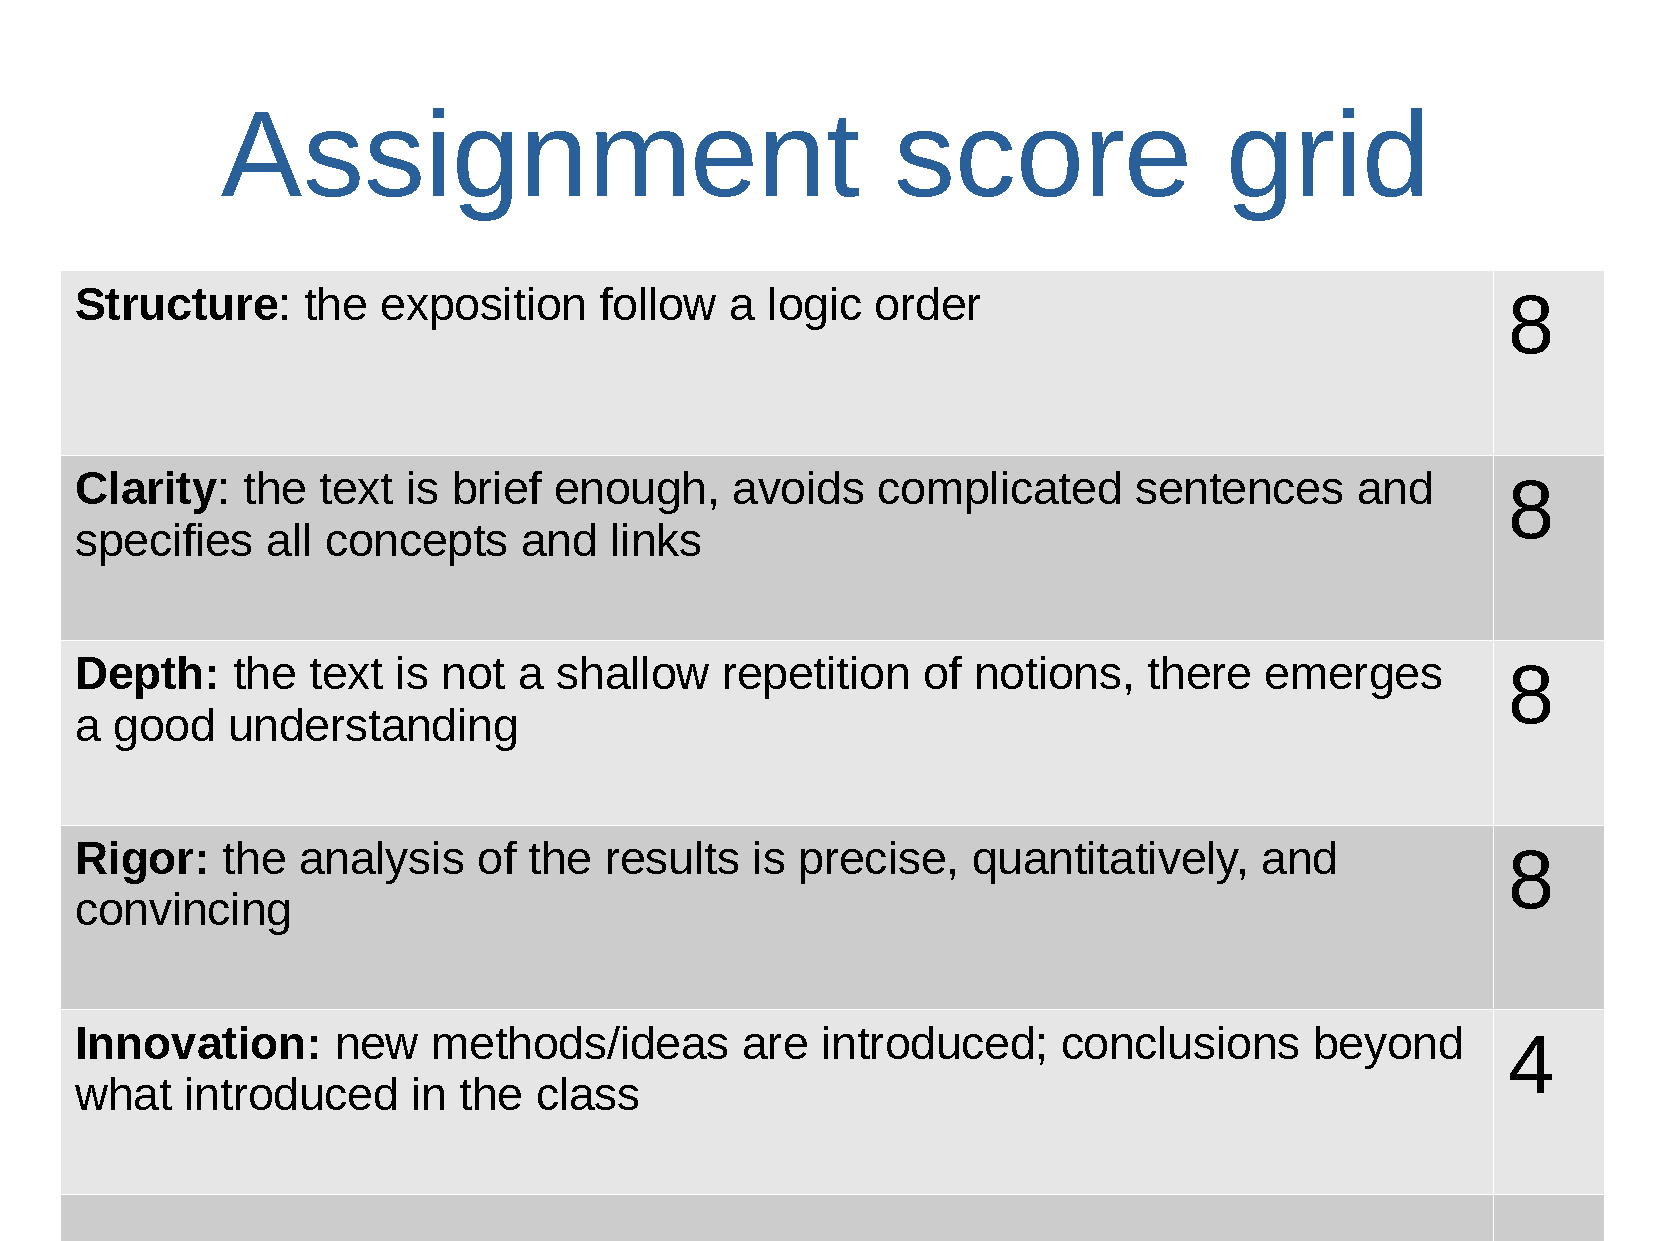
\includegraphics[width=\textwidth]{description_assignment_LCPB_20-21.pdf}
\end{figure*}
%%%%%%%%%%%%%%%%%%%


\end{document}





























